\documentclass[tikz,border=10pt]{standalone}
% Scale s = 0.017978 cm/px, origin at A (px 142,349); y flipped
\begin{document}
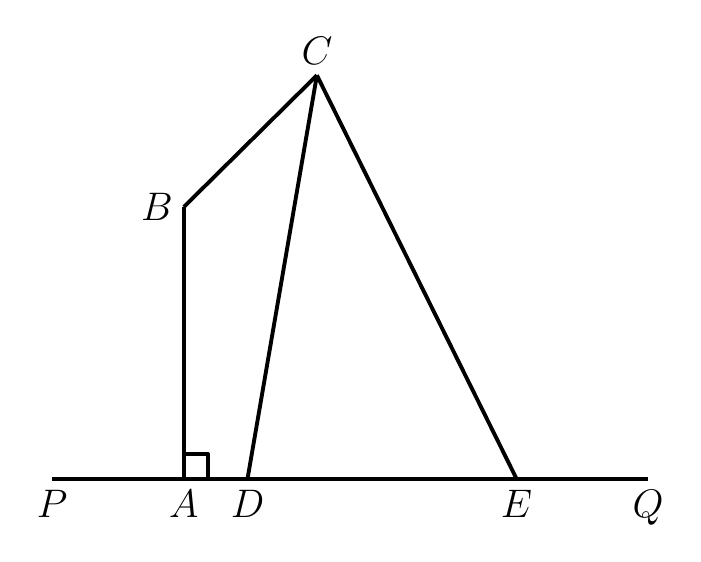
\begin{tikzpicture}[line width=1.4pt, line join=round, font=\fontsize{14}{16.8}\selectfont]
  % Named coordinates (cm)
  \coordinate (P) at (-1.672,0);
  \coordinate (A) at (0,0);
  \coordinate (D) at (0.809,0);
  \coordinate (E) at (4.225,0);
  \coordinate (Q) at (5.896,0);
  \coordinate (B) at (0,3.452);
  \coordinate (C) at (1.690,5.124);

  % Horizontal line PQ
  \draw (P) -- (Q);

  % Segments
  \draw (A) -- (B);
  \draw (B) -- (C);
  \draw (C) -- (D);
  \draw (C) -- (E);

  % Right-angle mark at A, inside the angle toward D and B
  \draw (0.31,0) -- (0.31,0.31) -- (0,0.31);

  % Labels
  \node[left] at (B) {$B$};
  \node[above] at (C) {$C$};
  \node[below] at (P) {$P$};
  \node[below] at (A) {$A$};
  \node[below] at (D) {$D$};
  \node[below] at (E) {$E$};
  \node[below] at (Q) {$Q$};
\end{tikzpicture}
\end{document}